\ifpdf
\graphicspath{ {Chapters/DrellYan/Figs/} }
\section{Drell-Yan}

%\begin{frame}[label=current]
\begin{frame}
  \frametitle{Drell-Yan}

  \setlength\abovecaptionskip{-3pt}
  \setlength{\belowcaptionskip}{-25pt}
  \begin{columns}
    \column{0.47\textwidth}
    \begin{figure}
      \vspace*{-1.2cm}
      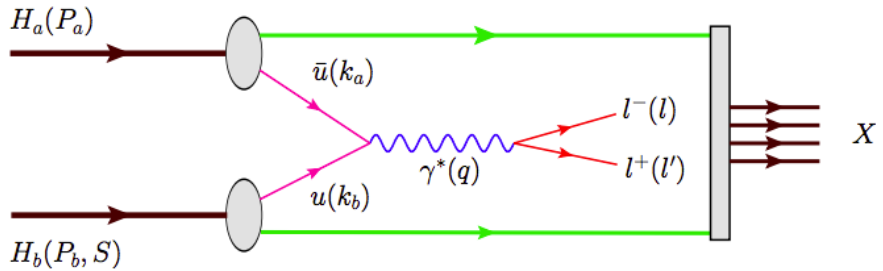
\includegraphics[width=\textwidth]{DY_feyDiagram}
      \caption{The Drell-Yan process Feynman diagram}
    \end{figure}
    \column{0.47\textwidth}
    \begin{figure}
      \vspace*{-1.2cm}
      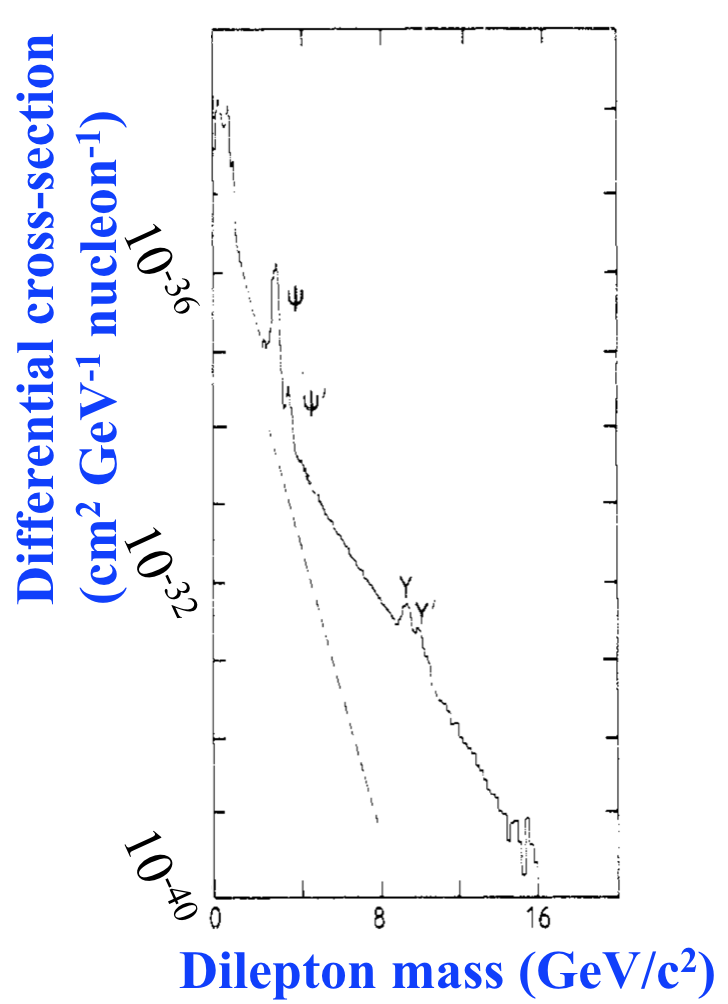
\includegraphics[width=0.8\textwidth]{DY_diffXsection}
      %\caption{The Drell-Yan differential cross-section}
    \end{figure}  
  \end{columns}
  
  \begin{subequations}
    \vspace*{-0.6cm}
    \begin{align*}
      &x_{a(b)} = \frac{q^2}{P_{a(b)} \cdot q} & \text{x-Bjorken,
        parton longitudinal momentum fraction.}\\ &M_{\mu\bar{\mu}}^2 = q^2 = Q^2 = sx_ax_b
      & \text{Invariant mass of the virtual photon.}
    \end{align*}
  \end{subequations}
  
  \begin{itemize}
  \item Describes the process where the final state results in 2
    leptons
  \item Rapid drop off of cross-section as a function of Q$^2$
  \end{itemize}
\end{frame}


%\begin{frame}[label=current]
\begin{frame}
  \frametitle{DY cross-section}

  \begin{itemize}
  \item The spin-dependent Drell-Yan cross-section gives access to an
    amplitude related to the Sivers function
  \end{itemize}
  \begin{equation*}
    \mathrm{d}\sigma_{DY}^{\uparrow} \propto \|S_T \|
    \color{red}A_T^{\sin(\phi_S)}\color{black}\sin(\phi_S) \qquad
    \qquad \color{red}A_T^{\sin(\phi_S)} \color{black} \propto
    \text{Sivers(proton)}
  \end{equation*}

  \begin{columns}
    \column{0.5\textwidth}
    \begin{figure}
      \centering
      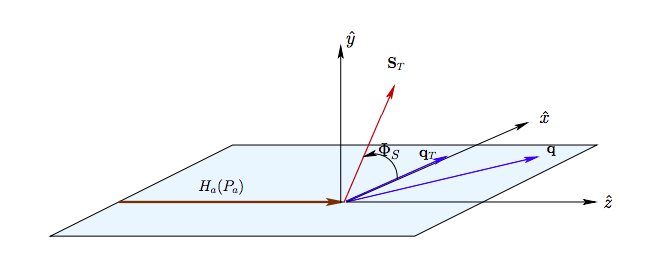
\includegraphics[width=\textwidth]{TargFrame}
      \caption{Target reference frame}
    \end{figure}
    \column{0.5\textwidth}
    \begin{figure}
      \centering
      \includegraphics[width=\textwidth]{CSFrame}
      \caption{Collins-Soper center of momentum reference frame}
    \end{figure}
  \end{columns}
\end{frame}


%\subsection{Kinematics}
\begin{frame}
  \frametitle{COMPASS Drell-Yan Kinematics}

  \begin{figure}
    \centering
    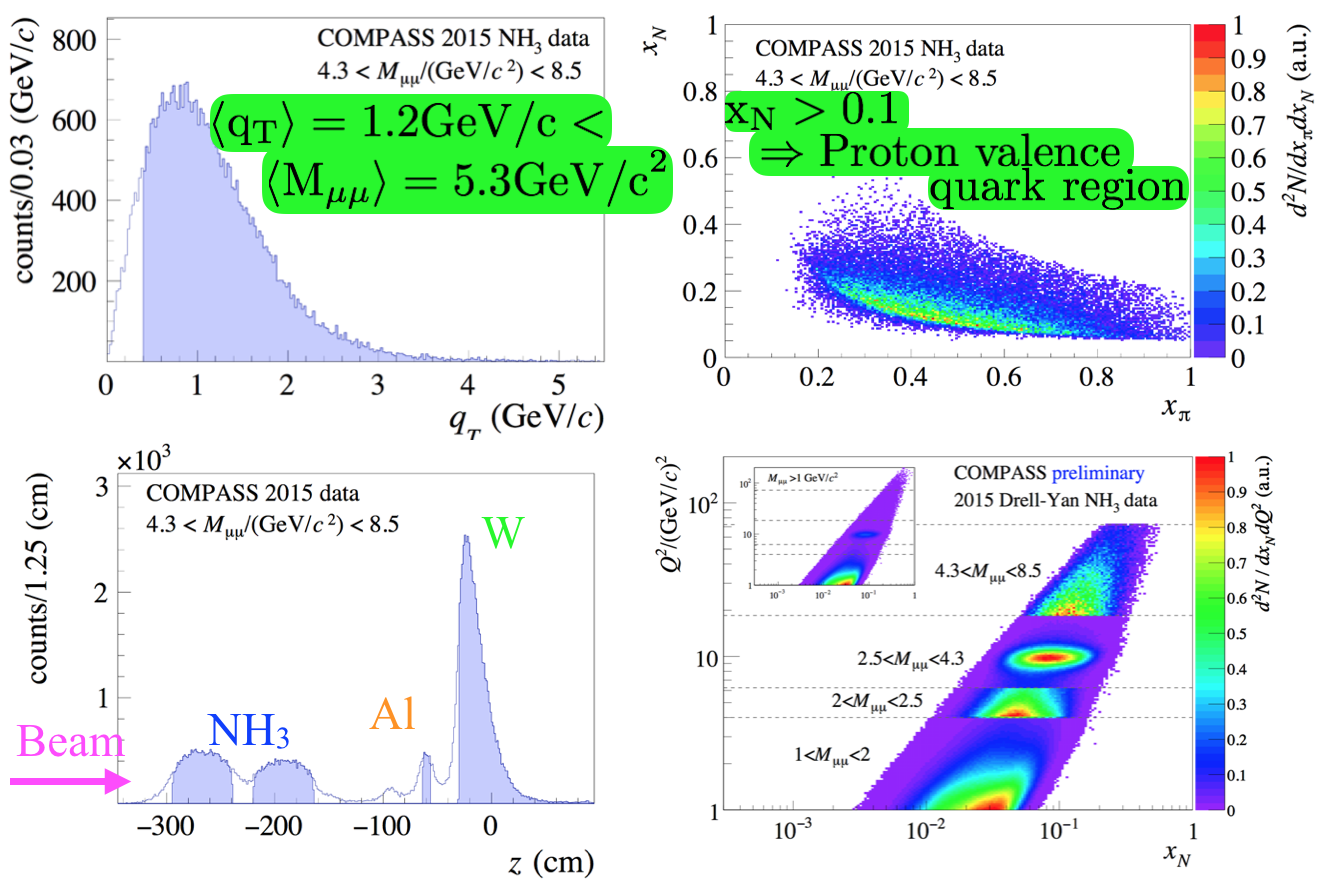
\includegraphics[width=0.9\textwidth]{Kinematics}
  \end{figure}
\end{frame}
